%----------------------------------------------------------------------------------------
%    PACKAGES AND THEMES
%----------------------------------------------------------------------------------------

\documentclass[aspectratio=169,xcolor=dvipsnames]{beamer}
\usetheme{SimpleDarkBlue}

\usepackage{hyperref}
\usepackage{graphicx} % Allows including images
\usepackage{booktabs} % Allows the use of \toprule, \midrule and \bottomrule in tables
\usepackage{subcaption}
\usepackage{color,soul}
\usepackage{multirow}

%----------------------------------------------------------------------------------------
%    TITLE PAGE
%----------------------------------------------------------------------------------------

\title{Leveraging Alternative Data for Mixed Martial Arts Betting Markets}
\subtitle{Yale Sports Analytics}

\author{Eugene Han}

\institute
{
    Department of Statistics \& Data Science \\
    Yale University % Your institution for the title page
}
\date{April 18, 2025} % Date, can be changed to a custom date

%----------------------------------------------------------------------------------------
%    PRESENTATION SLIDES
%----------------------------------------------------------------------------------------

\begin{document}

\begin{frame}
    % Print the title page as the first slide
    \titlepage
\end{frame}

%------------------------------------------------

\begin{frame}{Mixed Martial Arts (MMA)}
    \begin{itemize}
        \item ``Hybrid combat sport incorporating techniques from boxing, wrestling, judo, jujitsu, karate, Muay Thai (Thai boxing), and other disciplines"

        \item Ultimate Fighting Championship (UFC) is the largest global promotion $\rightarrow$ focus of this project
    \end{itemize}
    \begin{figure}
        \centering
        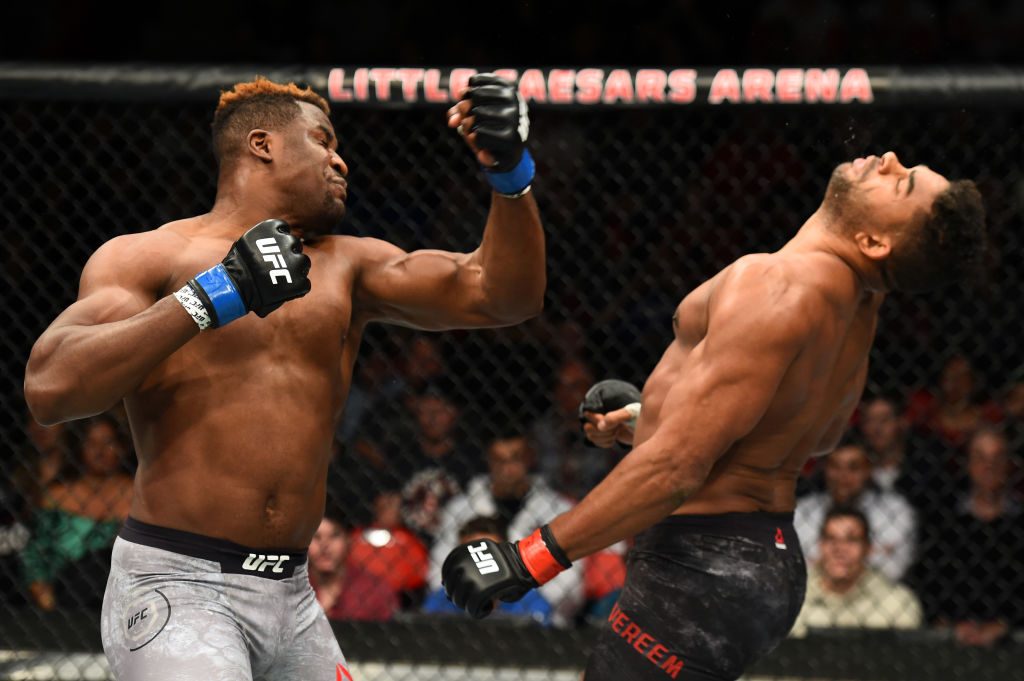
\includegraphics[width=0.5\linewidth]{figures/mma_ko.png}
    \end{figure}
\end{frame}

%------------------------------------------------

\begin{frame}{Sports Betting}
    \begin{itemize}
        \item Moneyline bets: wagers placed on a game’s outcome, i.e. who will win
        \begin{itemize}
            \item Voided if there is no winner
        \end{itemize}

        \item Odds are a dual representation
        \begin{itemize}
            \item Payouts

            \item Implied probabilities
        \end{itemize}

        \item Example: Fighter A ($+150$) vs. Fighter B ($-170$)
        \begin{itemize}
            \item $\$2.50$ returned for every $\$1$ wagered if fighter A wins, implies $40\%$ win chance

            \item $\$1.59$ returned for every $\$1$ wagered if fighter B wins, implies $63\%$ win chance

            \item House edge of $3\%$
        \end{itemize}

        \begin{alertblock}{Main Takeaway}
            Beating the market is a \textit{\textbf{probabilistic}} problem!
        \end{alertblock}
    \end{itemize}
\end{frame}

%------------------------------------------------

\begin{frame}{Problem Definition}
    For a given fight $i$, let $Y_i$ be defined as
    $$Y_i = \begin{cases}
        1 & \text{if the red corner fighter wins} \\
        0 & \text{if the blue corner fighter wins}
    \end{cases}$$

    We want to
    \begin{enumerate}
        \item Model $\mathbb{P}(Y_i = 1 \mid X_i)$ using information known strictly before the event

        \item Place bets when our model's predicted probabilities disagree with those implied by the betting market
    \end{enumerate}
\end{frame}

%------------------------------------------------

\begin{frame}{Previous Works}
    \begin{itemize}
        \item Some existing work, mostly amateur projects
    
        \item Common limitations:
        \begin{itemize}
            \item Almost exclusively uses UFC Stats, the official data provider of the UFC

            \item Methodology issues with modeling and/or feature engineering 

            \item No attention to calibration (e.g., do model's probabilities actually reflect confidence/empirical proportions?)

            \item Unrealistic backtesting setups, too small of sample sizes 
        \end{itemize}

        \item How can we improve on this?
    \end{itemize}
\end{frame}

%------------------------------------------------

\begin{frame}{Innovations}
    \begin{enumerate}
        \item Novel dataset incorporating ``alternative" (i.e. nontraditional) data sources

        \item Rigorous backtesting over 8 years with hypothesis testing

        \item Experimenting with ideas from conformal prediction framework and robust optimization for betting under uncertainty
    \end{enumerate}
\end{frame}

%------------------------------------------------

\begin{frame}{The Dataset}
    \begin{table}[]
    \begin{tabular}{@{}ll@{}}
    \toprule
    Source          & Examples of Data                            \\ \midrule
    UFC Stats       & Per-round striking/grappling stats          \\
    ESPN            & Additional bout-aggregated striking/grappling stats         \\
    Wikipedia       & Event attendance, venue location/capacity   \\
    Sherdog         & Fighters' full professional fight histories \\
    Fight Matrix    & Custom monthly rankings and Elo-like rating scores           \\
    Tapology        & Weigh-in results, gym/team affiliations     \\
    MMA Decisions   & Per-round scoring by judge                  \\
    Best Fight Odds & Historical timestamped betting odds for older events        \\
    FightOdds.io    & Historical betting odds for recent years, fighting styles           \\
    Bet MMA         & Weight misses, short notice fights          \\ \bottomrule
    \end{tabular}
    \caption{Overview of data sources}
    \end{table}
\end{frame}

%------------------------------------------------

\begin{frame}{The Dataset (cont.)}
    \begin{itemize}
        \item About 2 to 2.5 months of work
        \begin{itemize}
            \item Scraping, cleaning, cross-source ID matching
        \end{itemize}

        \item Relational database design (SQL $>$ CSVs/data frames)
        \begin{itemize}
            \item 58 tables

            \item 6.9 million rows

            \item 64.7 million individual data points

            \item 411 MB, over $50 \times$ bigger than UFC Stats alone ($\sim 8$ MB)
        \end{itemize}

        \item Completely open-source
    \end{itemize}
\end{frame}

%------------------------------------------------

\begin{frame}{Feature Engineering}
    \begin{itemize}
        \item ``Kitchen sink" approach: Generate tons of candidates, throw away most later
        \begin{itemize}
            \item Mostly based on domain knowledge/intuition
            \item Semi-systematic
        \end{itemize}

        \item Three ``groupings"
        \begin{itemize}
            \item \textbf{Event-Level}: Shared attributes across same-event fights (e.g., venue elevation)

            \item \textbf{Bout-Level}: Attributes of individual fights (e.g., weight class)

            \item \textbf{Fighter-Level}: Comparative measures based on fighters' attributes and past performance (e.g., difference in historical strikes landed per second)
        \end{itemize}

        \item \textbf{Important}: All features were created respecting temporal order
    \end{itemize}
\end{frame}

%------------------------------------------------

\begin{frame}{Feature Engineering (cont.)}
    \begin{figure}
    \centering
    \begin{subfigure}{.45\textwidth}
      \centering
      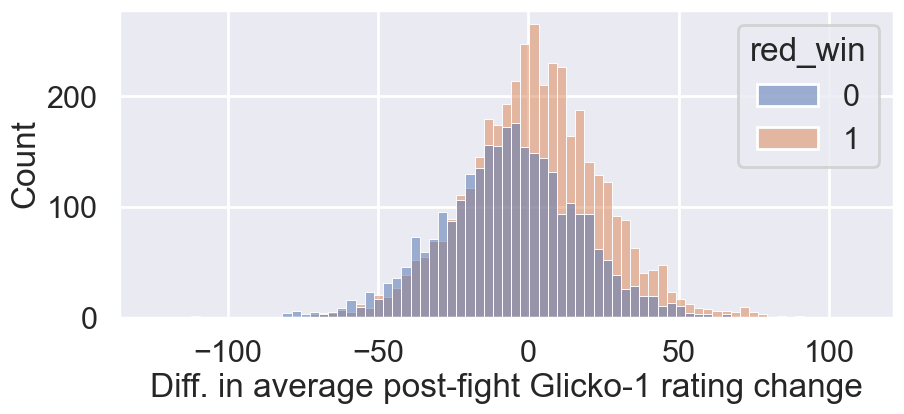
\includegraphics[width=\linewidth]{figures/glicko_1.png}
      % \caption{A subfigure}
      % \label{fig:sub1}
    \end{subfigure}
    \begin{subfigure}{.45\textwidth}
      \centering
      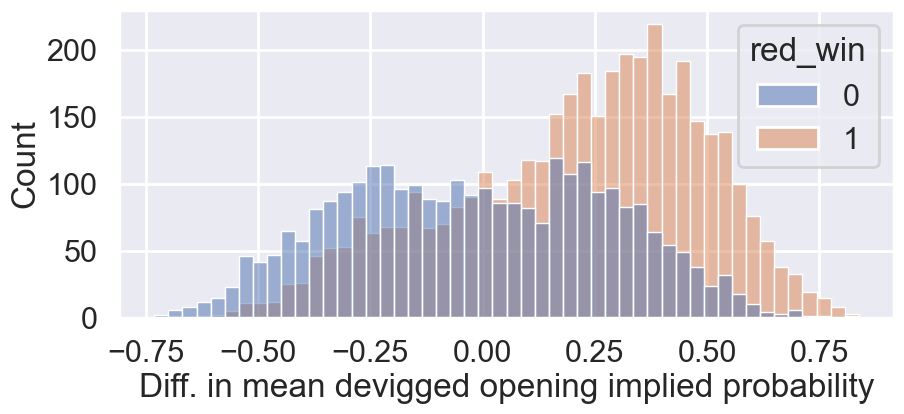
\includegraphics[width=\linewidth]{figures/opening_implied.png}
      % \caption{A subfigure}
      % \label{fig:sub2}
    \end{subfigure}
    \caption{Class distributions for example fighter-level features}
    \end{figure}
\end{frame}

%------------------------------------------------

\begin{frame}{Modeling}
    \begin{itemize}
        \item Four-step approach
        \begin{enumerate}
             \item \textbf{Odds Feature Ablation}: Inclusion/exclusion of opening odds-derived feature

            \item \textbf{Feature Selection}: Variance thresholding followed by top K selection via mutual information scores
    
            \item \textbf{Base Model}: Experimented with ridge logistic regression and gradient boosting
    
            \item \textbf{Calibration}: Inclusion/exclusion of using Venn-Abers predictors, which outputs an interval $(p_0, p_1)$ with validity guarantees such that
            $p_0 \leq \mathbb{P}(y = 1 \mid x) \leq p_1$ (informally)
        \end{enumerate}

        \item Total of 8 model pipelines

        \item Hyperparameter tuning
        \begin{itemize}
            \item Model parameters and K

            \item Stratified 10-fold CV

            \item Bayesian optimization with Optuna

            \item Optimize for log loss
        \end{itemize}
    \end{itemize}
\end{frame}

%------------------------------------------------

\begin{frame}{Bet Sizing}
    \begin{itemize}
        \item Suppose an event has $m$ fights
        \begin{itemize}
            \item These are essentially fought back-to-back

            \item We want to place all our bets at once
        \end{itemize}

        \item $2^m$ different outcome sequences (ignoring draws, no contests)

        \item $2m + 1$ bets
        \begin{itemize}
            \item One bet per fighter

            \item A risk-free ``no-bet" option that returns the full wager w.p. $1$
        \end{itemize}

        \item How should one allocate their money?
        \begin{itemize}
            \item One option is to optimize for the growth rate of capital

            \item This has some desirable properties (e.g., has an expected time to reach a specified goal that is asymptotically less than any other strategy)
        \end{itemize}
    \end{itemize}
\end{frame}

%------------------------------------------------

\begin{frame}{Simultaneous (``Classical") Kelly}
    \begin{itemize}
        \item For returns matrix $R \in \mathbb{R}^{(2m + 1) \times 2^m}$ and outcome probabilities $\pi \in \Delta_{2^m}$, we want to find allocation $b \in \mathbb{R}^{2 m + 1}_{\geq 0}$ to maximize the expected log growth rate of wealth, $G_{\pi} (b) = \pi^T \log(R^Tb)$:
        $$\begin{aligned}
        \max_{b} \quad & \pi^T \log(R^Tb) \\
        \textrm{s.t.} \quad & 1^T b = 1 \\
                            & b \geq 0
        \end{aligned}$$

        \item Ex. For $m = 2$, construct $R$ and estimate $\pi$ as
        $$R = \begin{pmatrix}
        o_{r, 1} & o_{r, 1} & 0 & 0 \\
        0 & 0 & o_{b, 1} & o_{b, 1} \\
        o_{r, 2} & 0 & o_{r, 2} & 0 \\
        0 & o_{b, 2} & 0 & o_{b, 2} \\
        1 & 1 & 1 & 1
        \end{pmatrix}, \quad \hat{\pi} = \begin{pmatrix}
            \hat{p}_1 \hat{p}_2 \\
            \hat{p}_1 (1 - \hat{p}_2) \\
            (1 - \hat{p}_1) \hat{p}_2 \\
            (1 - \hat{p}_1) (1 - \hat{p}_2)
        \end{pmatrix}$$
        given odds $o_{r} = (o_{r,1}, \ldots, o_{r,m})$ , $o_b = (o_{b,1}, \ldots, o_{b,m})$ and $\hat{p}_j = \hat{\mathbb{P}}(Y_j = 1 \mid X_j)$
    \end{itemize}
\end{frame}

%------------------------------------------------

\begin{frame}{Distributional Robust Kelly}
    \begin{itemize}
        \item Maximize expected worst case log growth rate, $G_{\Pi}(b) = \inf_{\pi \in \Pi} G_{\pi} (b)$, over uncertainty set $\Pi = \{\pi \in \Delta_{2^m} \mid A \pi \leq d \}$:
        $$\begin{aligned}
            \max_{b, \lambda} \quad & \min(\log(R^T b) +  A^T \lambda)  - d^T \lambda\\
            \textrm{s.t.} \quad & 1^T b = 1 \\
                                & b \geq 0 \\
                                & \lambda \geq 0
        \end{aligned}$$

        \item Construct $A$ and $d$ as
        $$A = \begin{pmatrix}
            - I_{2^m} \\
            I_{2^m}
        \end{pmatrix}, \quad d = \begin{pmatrix}
            -\hat{\pi}_{\text{lower}} \\
            \hat{\pi}_{\text{upper}}
        \end{pmatrix}$$
        where $\hat{\pi}_{\text{lower}}, \hat{\pi}_{\text{upper}}$ are defined like $\hat{\pi}$ using the $(p_0, p_1)$ outputs from Venn-Abers
    \end{itemize}
\end{frame}

%------------------------------------------------

\begin{frame}{Backtesting Setup}
    \begin{itemize}
        \item 8-year backtest period
        \begin{itemize}
            \item Start of 2017 to end of 2024

            \item 3960 bouts, 331 events
        \end{itemize}

        \item Model pipelines are refit after every event, hyperparameters retuned at the end of each year

        \item Initial bankroll of $\$1000$

        \item Closing odds from Bovada Sportsbook used to determine wagers
        \begin{itemize}
            \item $\$0.50$ minimum bet size $\Longrightarrow$ all bets less than $\$0.50$ rounded down to $\$0$

            \item Draws and no contests return full corresponding wager
        \end{itemize}

        \item Model pipelines with Venn-Abers combined with both betting strategies
        \begin{itemize}
            \item Total of 12 model pipeline and betting strategy combinations

            \item Total of 36 combinations when considering different fractions
        \end{itemize}
    \end{itemize}
\end{frame}

%------------------------------------------------

\begin{frame}{Monte Carlo Hypothesis Testing}
    \begin{itemize}
        \item How do we know our observed profit is not by chance?

        \item Under null hypothesis, our approach has no edge $\Longleftrightarrow$ closing odds reflect the true outcome probabilities
        \begin{enumerate}
            \item Compute devigged implied probabilities (normalize to remove house edge)

            \item Sample outcome sequences according to these probabilities

            \item Compute profit/loss in this simulated reality

            \item Repeat a lot of times (10000)
        \end{enumerate}

        \item Calculate p-value as
        $$\text{p-value} = \frac{(\text{\# of simulations with profit}\geq\text{observed}) + 1}{(\text{total \# of simulations}) + 1}$$
        and adjust using a Bonferroni correction
    \end{itemize}
\end{frame}

%------------------------------------------------

\begin{frame}{Model Results}
    \begin{table}[]
    \begin{tabular}{@{}lrr@{}}
    \toprule
    Model Pipeline                           & Log Loss          & Brier Score       \\ \midrule
    Logistic Regression                      & \hl{0.608060} & 0.210443 \\
    Logistic Regression (No Odds)            & 0.629998          & 0.220371          \\
    Venn-Abers Logistic Regression           & 0.608881          & 0.210849          \\
    Venn-Abers Logistic Regression (No Odds) & 0.632596          & 0.221477          \\
    LightGBM                                 & 0.611128          & 0.211772          \\
    LightGBM (No Odds)                       & 0.631593          & 0.221174          \\
    Venn-Abers LightGBM                      & 0.611205          & 0.211956          \\
    Venn-Abers LightGBM (No Odds)            & 0.633977          & 0.222121          \\ \midrule
    \textit{Bovada Sportsbook}               & \textit{0.608142} & \hl{\textit{0.210265}} \\ \bottomrule
    \end{tabular}
    \caption{Summary of model metrics over the backtest period, compared with closing odds}
    \end{table}
\end{frame}

%------------------------------------------------

\begin{frame}{Model Results (cont.)}
    \begin{figure}
        \centering
        \captionsetup{justification=centering}
        \begin{subfigure}{.24\linewidth}
            \centering
            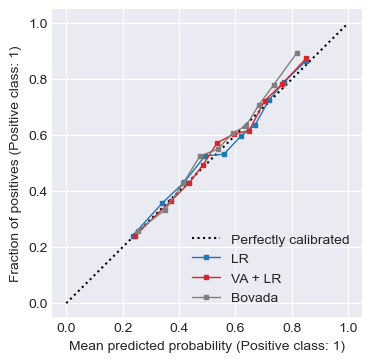
\includegraphics[width=\linewidth]{figures/lr_and_va.png}
        \end{subfigure}
        \begin{subfigure}{.24\linewidth}
            \centering
            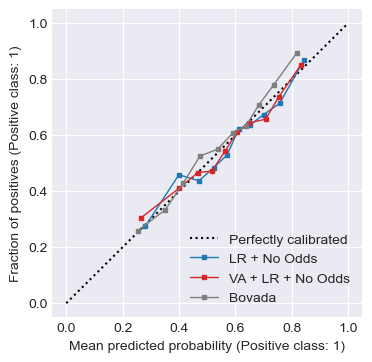
\includegraphics[width=\linewidth]{figures/lr_no_odds_and_va.png}
        \end{subfigure}
        \begin{subfigure}{.24\linewidth}
            \centering
            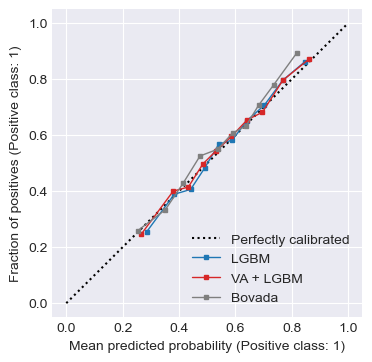
\includegraphics[width=\linewidth]{figures/lightgbm_and_va.png}
        \end{subfigure}
        \begin{subfigure}{.24\linewidth}
            \centering
            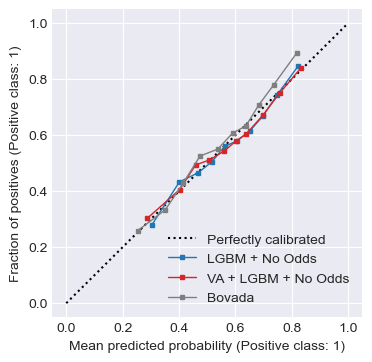
\includegraphics[width=\linewidth]{figures/lightgbm_no_odds_and_va.png}
        \end{subfigure}
        \caption{Calibration plots comparing model pipelines with and without Venn-Abers}
    \end{figure}
\end{frame}

%------------------------------------------------

\begin{frame}{Betting Results}
    \tiny
    \begin{table}[]
    \begin{tabular}{@{}llrrrrrr@{}}
    \toprule
    Model Pipeline                                            & Betting Strategy                    & Fraction & Profit (\$) & Total Bets & Yield (\%) & MDD (\%) & Adj. p-value        \\ \midrule
    \multirow{3}{*}{Logistic Regression}                      & \multirow{3}{*}{Simultaneous} & 0.10     & 1318.98     & 1178       & 6.40       & -22.04            & \multirow{3}{*}{\textbf{0.0516}} \\
                                                              &                                     & 0.15     & 2159.40     & 1196       & 5.25       & -32.02            &                           \\
                                                              &                                     & 0.25     & \textbf{3763.63}     & 1201       & 3.47       & -50.46            &                           \\
    Logistic Regression (No Odds)                             & Simultaneous                  & 0.10     & -114.95       & 1810       & -0.53       & -40.19            & 0.9083                  \\
    \multirow{2}{*}{Venn-Abers Logistic Regression}           & Simultaneous                  & 0.10     & 430.80      & 1445       & 2.24       & -34.74            & 0.3528                  \\
                                                              & Distrib. Robust        & 0.10     & 338.04      & 609        & \textbf{7.47}       & \textbf{-16.36}            & 0.3780                  \\
    \multirow{2}{*}{Venn-Abers Logistic Regression (No Odds)} & Simultaneous                 & 0.10     & -181.54      & 1865       & -0.78      & -45.45            & 1.0000                  \\
                                                              & Distrib. Robust         & 0.10     & -260.40     & 1396       & -2.28      & -34.03            & 1.0000                  \\
    LightGBM                                                  & Simultaneous                 & 0.10     & 192.37      & 1610       & 0.89       & -49.20            & 0.5999                  \\
    LightGBM (No Odds)                                        & Simultaneous                 & 0.10     & -584.14     & 1906       & -3.29      & -68.99            & 1.0000                  \\
    \multirow{2}{*}{Venn-Abers LightGBM}                      & Simultaneous                  & 0.10     & 258.96      & 1540       & 1.21       & -46.78            & 0.5111                  \\
                                                              & Distrib. Robust       & 0.10     & 130.44      & 881        & 1.93       & -30.03            & 1.0000                  \\
    \multirow{2}{*}{Venn-Abers LightGBM (No Odds)}            & Simultaneous                 & 0.10     & -551.64     & 1894       & -2.86      & -72.54            & 1.0000                  \\
                                                              & Distrib. Robust        & 0.10     & -394.33     & 1380      & -2.57      & -62.51            & 1.0000                  \\ \bottomrule
    \end{tabular}
    \caption{Betting metrics by model pipeline and betting strategy combination}
    \end{table}
    \normalsize
\end{frame}

%------------------------------------------------

\begin{frame}{Betting Results (cont.)}
    \begin{figure}[!htb]
    \centering
    \captionsetup{justification=centering}
    \begin{subfigure}{.3\linewidth}
      \centering
      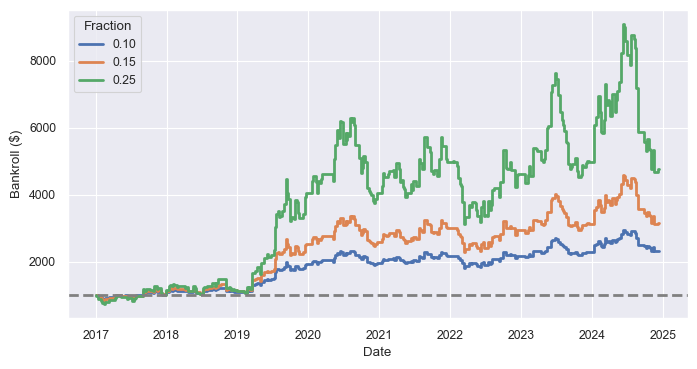
\includegraphics[width=\linewidth]{figures/bankroll_lr_simultaneous.png}
      \caption{Logistic regression}
    \end{subfigure}%
    \begin{subfigure}{.3\linewidth}
      \centering
      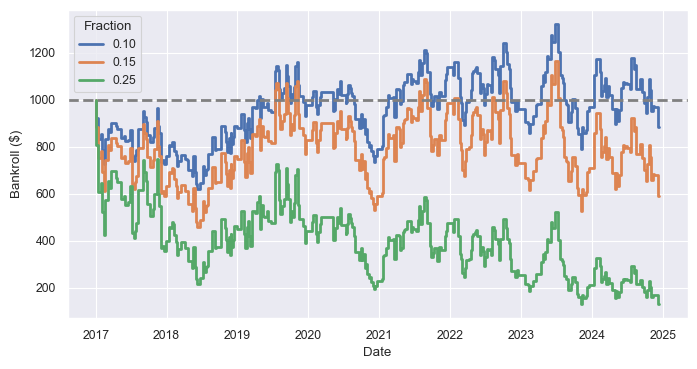
\includegraphics[width=\linewidth]{figures/bankroll_lr_no_odds_simultaneous.png}
      \caption{Logistic regression, no odds}
    \end{subfigure}
    \caption{Bankroll over time for selected simultaneous Kelly strategy combinations}
    \end{figure}

    \begin{figure}[!htb]
        \centering
        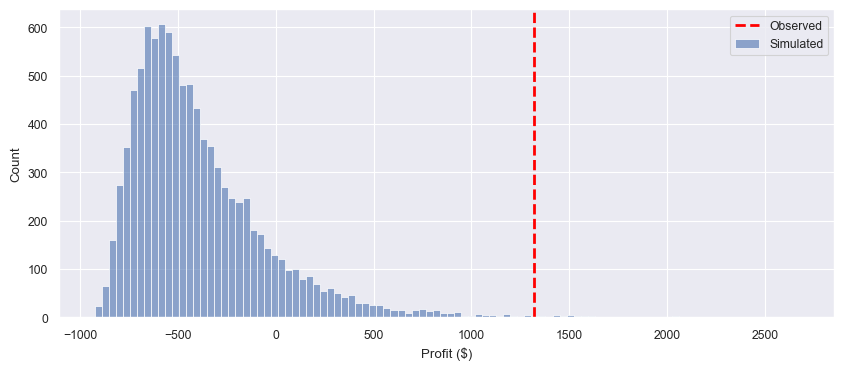
\includegraphics[width=.4\linewidth]{figures/mc_results.png}
        \caption{Simulated profit vs. observed, LR and simultaneous Kelly $(f = 0.10)$}
    \end{figure}
\end{frame}

%------------------------------------------------

\begin{frame}{Case Study: Logistic Regression and Simultaneous Kelly}
    \begin{itemize}
        \item Clearly, logistic regression with simultaneous Kelly give the best results
        \begin{itemize}
            \item Concluding with this is boring
        \end{itemize}

        \item Further questions
        \begin{itemize}
            \item What features are driving these results?

            \item Why does most of our bankroll growth take place 2019 and 2020, but stagnate afterwards?

            \item What types of fights is our model struggling with and why?

            \item Can we identify a stricter subset of fights to further optimize profits?
        \end{itemize}
    \end{itemize}
\end{frame}

%------------------------------------------------

\begin{frame}{Case Study (cont.)}
    \begin{itemize}
        \item Opening odds-derived feature at top, but importantly does not dominate the model

        \item Majority of features in top 20 are derived from sources other than UFC Stats
    \end{itemize}
    \begin{figure}
        \centering
        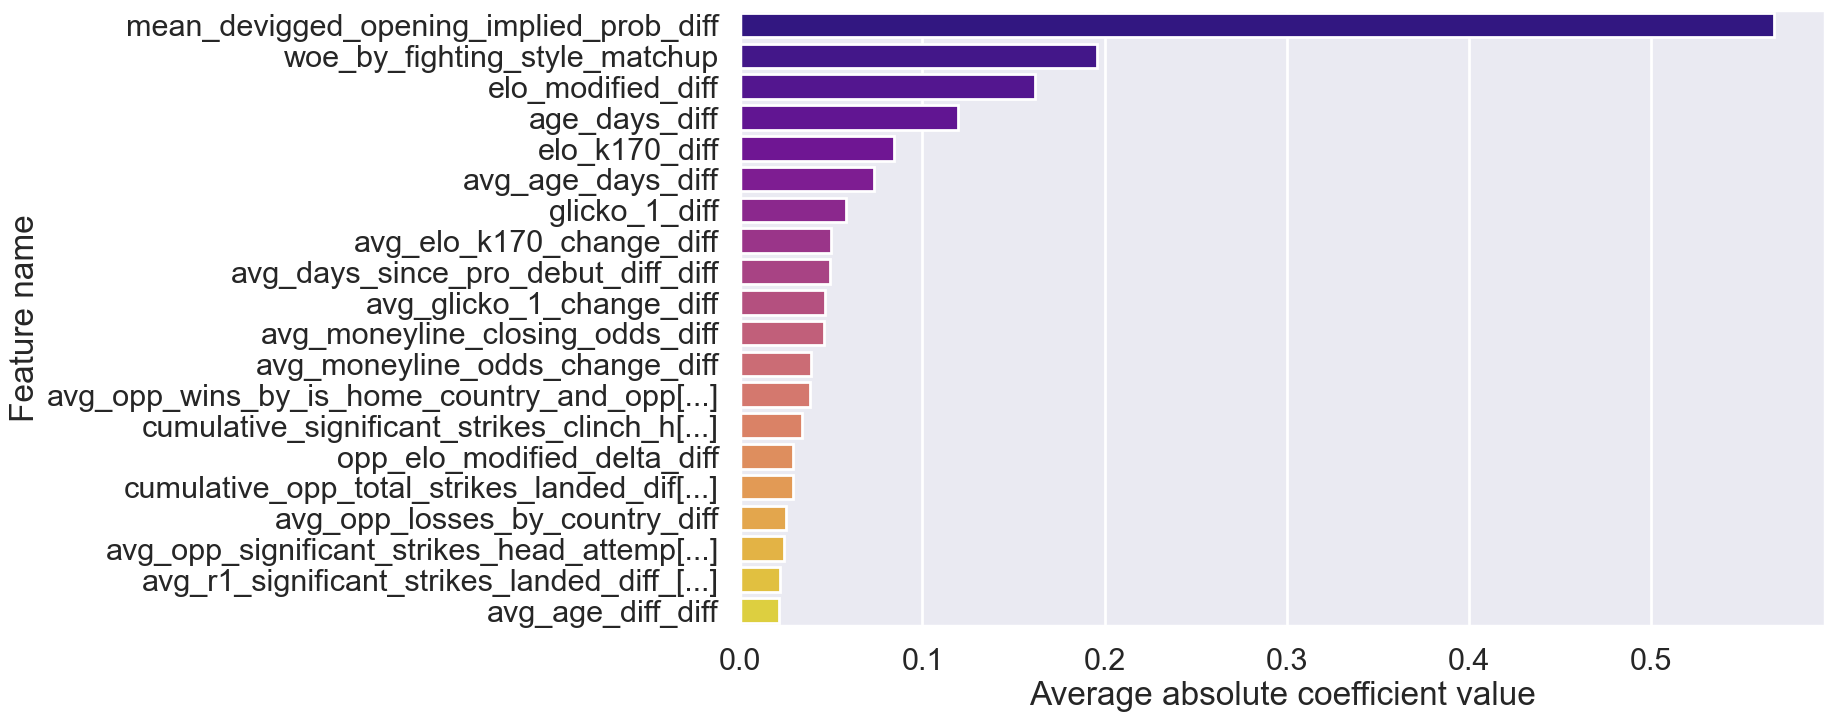
\includegraphics[width=0.65\linewidth]{figures/lr_feature_avg_abs_coef.png}
        \caption{Top 20 features by average absolute coefficient value in logistic regression model}
    \end{figure}
\end{frame}

%------------------------------------------------

\begin{frame}{Case Study (cont.)}
    \tiny
    \begin{table}[!htb]
    \centering
    \begin{tabular}{@{}cccrcccr@{}}
    \toprule
    \multirow{2}{*}{Year} & \multicolumn{3}{c}{Log Loss}                                                               & \multirow{2}{*}{}    & \multicolumn{3}{c}{Brier Score}                    \\ \cmidrule(lr){2-4} \cmidrule(l){6-8} 
                          & Model                        & Bovada                       & \multicolumn{1}{c}{$\Delta$} &                      & Model    & Bovada   & \multicolumn{1}{c}{$\Delta$} \\ \midrule
    2017                  & 0.614738                     & 0.609460                     & 0.005277                     &                      & 0.212572 & 0.210317 & 0.002256                     \\
    2018                  & \multicolumn{1}{l}{0.597811} & \multicolumn{1}{l}{0.597080} & 0.000731                     & \multicolumn{1}{l}{} & 0.206408 & 0.205833 & 0.000575                     \\
    2019                  & 0.624346                     & 0.636898                     & -0.012552                    &                      & 0.217742 & 0.223757 & -0.006016                    \\
    2020                  & 0.611094                     & 0.617461                     & -0.006367                    &                      & 0.211575 & 0.214045 & -0.002470                    \\
    2021                  & 0.622634                     & 0.621523                     & 0.001110                     &                      & 0.217409 & 0.216309 & 0.001100                     \\
    2022                  & 0.599701                     & 0.597913                     & 0.001788                     &                      & 0.207473 & 0.205662 & 0.001811                     \\
    2023                  & 0.608926                     & 0.602462                     & 0.006465                     &                      & 0.210956 & 0.207674 & 0.003282                     \\
    2024                  & 0.586208                     & 0.583386                     & 0.002822                     &                      & 0.199778 & 0.198925 & 0.000853                     \\ \bottomrule
    \end{tabular}
    \normalsize
    \caption{Model pipeline and sportsbook log loss and Brier score by year}
    \label{case_study_by_year}
    \end{table}

    \begin{figure}[!htb]
    \centering
    \captionsetup{justification=centering}
    \begin{subfigure}{0.3\linewidth}
      \centering
      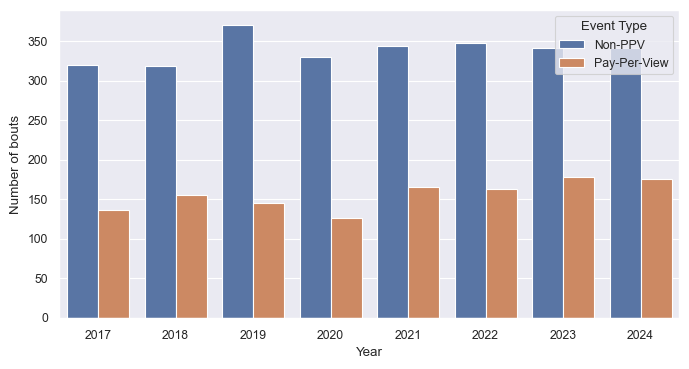
\includegraphics[width=\linewidth]{figures/event_type_by_year.png}
    \end{subfigure}
    \begin{subfigure}{0.3\linewidth}
      \centering
      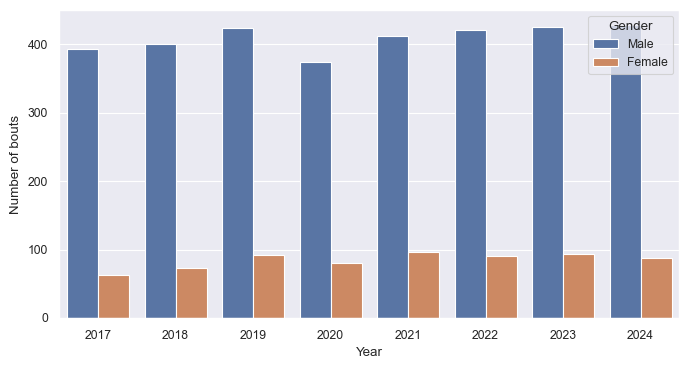
\includegraphics[width=\linewidth]{figures/gender_by_year.png}
    \end{subfigure}
    \begin{subfigure}{0.3\linewidth}
      \centering
      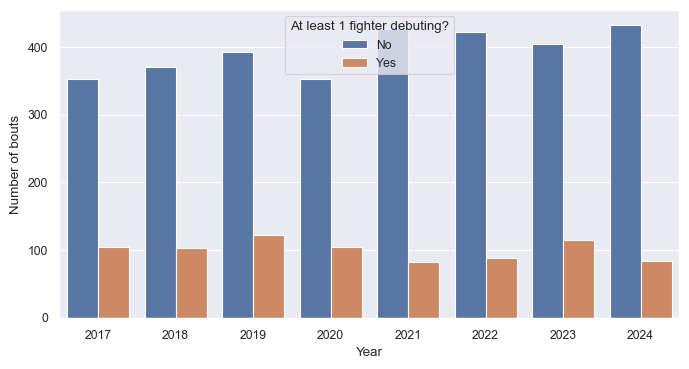
\includegraphics[width=\linewidth]{figures/debuts_by_year.png}
    \end{subfigure}
    \caption{Number of bouts per year by event type, gender, and debuts}
    \end{figure}
\end{frame}

%------------------------------------------------

\begin{frame}{Case Study (cont.)}
    \tiny
    \begin{table}[!htb]
    \centering
    \begin{tabular}{@{}cccrcccr@{}}
    \toprule
    \multirow{2}{*}{Event Type} & \multicolumn{3}{c}{Log Loss}                       & \multirow{2}{*}{} & \multicolumn{3}{c}{Brier Score}                    \\ \cmidrule(lr){2-4} \cmidrule(l){6-8} 
                            & Model    & Bovada   & \multicolumn{1}{c}{$\Delta$} &                   & Model    & Bovada   & \multicolumn{1}{c}{$\Delta$} \\ \midrule
    Pay-Per-View            & 0.593012 & 0.596247 & -0.003235                    &                   & 0.203459 & 0.204517 & -0.001057                    \\
    Non-PPV             & 0.614957 & 0.613594 & 0.001363                     &                   & 0.213644 & 0.212900 & 0.000744                     \\ \bottomrule
    \end{tabular}
    \normalsize
    % \caption{Model pipeline and sportsbook log loss and Brier score by event type}
    \end{table}

    \tiny
    \begin{table}[!htb]
    \centering
    \begin{tabular}{@{}cccrcccr@{}}
    \toprule
    \multirow{2}{*}{Gender} & \multicolumn{3}{c}{Log Loss}                       & \multirow{2}{*}{} & \multicolumn{3}{c}{Brier Score}                    \\ \cmidrule(lr){2-4} \cmidrule(l){6-8} 
                            & Model    & Bovada   & \multicolumn{1}{c}{$\Delta$} &                   & Model    & Bovada   & \multicolumn{1}{c}{$\Delta$} \\ \midrule
    Male                    & 0.603392 & 0.606017 & -0.002625                    &                   & 0.208329 & 0.209354 & -0.001025                    \\
    Female                  & 0.630458 & 0.618340 & 0.012118                     &                   & 0.220585 & 0.214636 & 0.005949                     \\ \bottomrule
    \end{tabular}
    \normalsize
    % \caption{Model pipeline and sportsbook log loss and Brier score by gender of both fighters}
    \end{table}

    \tiny 
    \begin{table}[!htb]
    \centering
    \begin{tabular}{@{}cccrcccr@{}}
    \toprule
    \multirow{2}{*}{UFC Experience} & \multicolumn{3}{c}{Log Loss}                       & \multirow{2}{*}{}    & \multicolumn{3}{c}{Brier Score}                    \\ \cmidrule(lr){2-4} \cmidrule(l){6-8} 
                                    & Model    & Bovada   & \multicolumn{1}{c}{$\Delta$} &                      & Model    & Bovada   & \multicolumn{1}{c}{$\Delta$} \\ \midrule
    Both debuting                   & 0.607946 & 0.579237 & 0.028709                     &                      & 0.210271 & 0.196018 & 0.014253                     \\
    One fighter debuting            & 0.573801 & 0.560372 & 0.013429                    & \multicolumn{1}{l}{} & 0.195112 & 0.189045 & 0.006067                     \\
    Both at least 1 fight           & 0.615511 & 0.619609 & -0.004098                    & \multicolumn{1}{l}{} & 0.213782 & 0.215412 & -0.001630                    \\
    Both at least 3 fights          & 0.614461 & 0.617389 & -0.002927                    & \multicolumn{1}{l}{} & 0.213161 & 0.214277 & -0.001116                    \\
    Both at least 5 fights          & 0.613856 & 0.617412 & -0.003556                    &                      & 0.212762 & 0.214238 & -0.001476                   \\ \bottomrule
    \end{tabular}
    \normalsize
    \caption{Model pipeline and sportsbook log loss and Brier score by event type, gender, and experience}
    \end{table}
\end{frame}

%------------------------------------------------

\begin{frame}{Case Study (cont.)}
    \begin{itemize}
        \item What if we ignore women's divisions and debuts?
        \item Rerun everything except on subset of original data

        \scriptsize
        \begin{table}[!htb]
        \centering
        \begin{tabular}{@{}lcc@{}}
        \toprule
                            & Log Loss & Brier Score \\ \midrule
        Logistic Regression & \hl{0.611250} & \hl{0.211724}    \\
        Bovada Sportsbook   & 0.616538 & 0.214093    \\ \bottomrule
        \end{tabular}
        \normalsize
        \caption{Model metrics over backtest period for fight subset, compared with closing odds}
        \end{table}

        \scriptsize
        \begin{table}[!htb]
        \centering
        \begin{tabular}{rrrrrr} 
        \toprule
        Fraction & Profit (\$) & Total Bets & Yield (\%) & MDD (\%) & Raw $p$-value            \\ 
        \toprule
        0.10     & 4758.95     & 964        & 15.99      & -20.56   & \multirow{3}{*}{0.0001}  \\
        0.15     & 11306.91    & 974        & 14.21      & -29.42   &                          \\
        0.25     & 43830.51    & 976        & 11.07      & -46.47   &                          \\
        \bottomrule
        \end{tabular}
        \normalsize
        \caption{Betting metrics by fraction, fight subset}
        \end{table}
    \end{itemize}
\end{frame}

%------------------------------------------------

\begin{frame}{Case Study (cont.)}
    \begin{figure}[!htb]
    \centering
    \captionsetup{justification=centering}
    \begin{subfigure}{.4\linewidth}
      \centering
      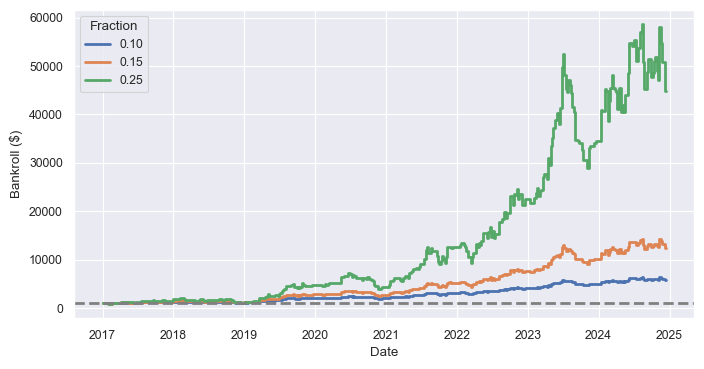
\includegraphics[width=\linewidth]{figures/bankroll_lr_case_study_simultaneous.png}
      % \caption{Bankroll over time by Kelly fraction}
    \end{subfigure}%
    \begin{subfigure}{.4\linewidth}
      \centering
      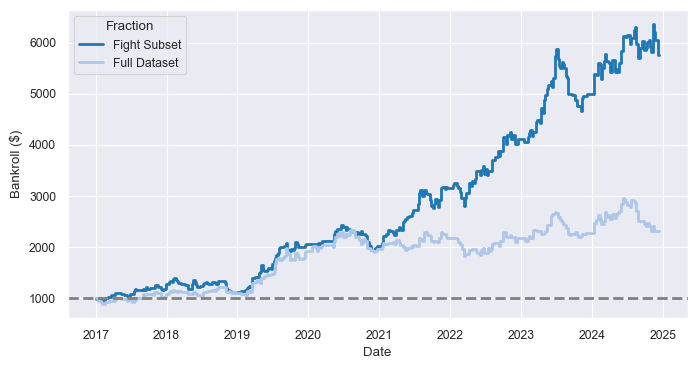
\includegraphics[width=\linewidth]{figures/bankroll_comparison.png}
      % \caption{Comparison for $f = 0.10$}
    \end{subfigure}
    \begin{subfigure}{.5\linewidth}
      \centering
      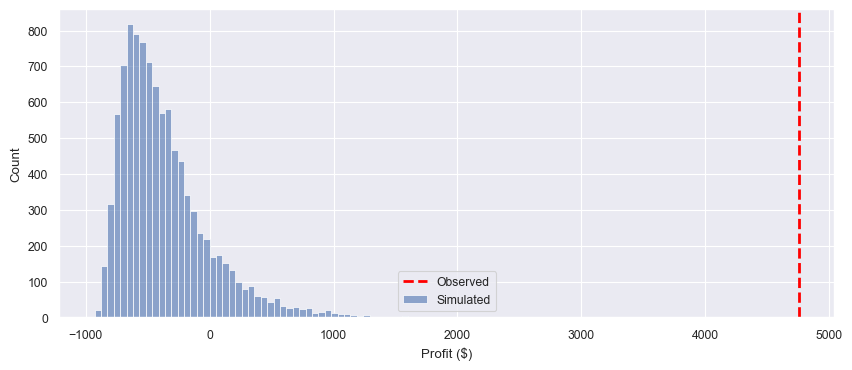
\includegraphics[width=\linewidth]{figures/mc_results_case_study.png}
      % \caption{Simulated profit vs. observed, $f = 0.10$}
    \end{subfigure}
    \caption{Selection of betting performance plots, fight subset}
    \end{figure}
\end{frame}

%------------------------------------------------

\begin{frame}{A Few Takeaways}
    \begin{itemize}
        \item Sportsbooks are difficult to beat
    
        \item Clear value-add from integrating alternative signals

        \item Market information is valuable

        \item Possible edge decay?
    \end{itemize}
\end{frame}

%------------------------------------------------

\begin{frame}{Future Work}
    \begin{itemize}
        \item Improvements to feature engineering and selection
        \begin{itemize}
            \item Time-weighted averages, Bayesian smoothing, genetic algorithms, etc.
        \end{itemize}

        \item Data source ablation studies
        \begin{itemize}
            \item Massive practical limitations imposed by having so many interdependencies
            \item Can we trim it down?
        \end{itemize}

        \item Collect even more data
        \begin{itemize}
            \item Theoretically possible to get timestamped odds data from FightOdds.io
        \end{itemize}

        \item Use dataset to answer other research questions
        \begin{itemize}
            \item What impact does elevation have on striking/grappling outputs?

            \item How do markets react to news such as late replacements, weight misses, etc.?

            \item To what extent does a fighter's ability to rehydrate and regain weight after weigh-ins affect their likelihood of winning?
        \end{itemize}
    \end{itemize}
\end{frame}

%------------------------------------------------

\begin{frame}{Miscellaneous}
    \begin{itemize}
        \item GitHub: \url{https://github.com/ehan03}
        \begin{itemize}
            \item Repository: \url{https://github.com/ehan03/yale-senior-thesis}
        \end{itemize}

        \item Tech stack
        \begin{itemize}
            \item Languages: Mainly Python, feature engineering in raw SQL

            \item Main libraries: Scrapy, Pandas, NumPy, Scikit-learn, LightGBM, Optuna, CVXPY, SQLite, SQLAlchemy, venn-abers (Ivan Petej), Seaborn
        \end{itemize}
    \end{itemize}
\end{frame}

%------------------------------------------------

\end{document}